\section{Platforma mobilna (Windows Mobile 6.1)}
\label{sec:wm-app}
Mobilne urządzenia przenośne z dnia na dzień zyskują na popularności. Każdego
dnia spotykamy się z nimi w domu, w pracy czy spacerując po parku. Z całą
pewnością można stwierdzić, iż większa część społeczeństwa obecnie jest w
posiadaniu telefonu komórkowego, komputera przenośnego czy też jakiegoś innego
urządzenia mobilnego. Wszystkie z wspomnianych urządzeń posiadają
charakterystyczną dla siebie platformę software'ową. Do najlepiej znanych we
współczesnym świecie zaliczyć można między innymi: Windows Mobile, iPhone,
BlackBerry, Symbian OS, Android, Maemo, OpenMoko itp. Każda z wymienionych
platform posiada inną genezę jak również ma swoje mocne i słabe strony.

Platformy takie jak Windows Mobile, BlackBerry czy iPhone ograniczone są do
urządzeń dedykowanych docelowo do współpracy z wspomnianymi środowiskami. Obok
różnorakich problemów z jakimi zmagają się wspomniane wcześniej platformy do
jednego z najpoważniejszych zaliczyć można bardzo ograniczone w niektórych
aspektach API\footnote{Application Programming Interface - interfejs
programowania aplikacji, specyfikacja instrukcji pozwalających na dostęp do
zasobów dostarczanych przez zewnętrzny program}. Nawet tak przenośna platforma
jak Java na urządzeniach przenośnych nie zawsze się sprawdza ze względu na liczne
braki oraz różnice w API zmuszające programistów do tworzenia kodu dedykowanego
dla konkretnego urządzenia. Symbian oraz Windows Mobile wypadają na tym tle nieco
lepiej ponieważ wspierają szerszą gamę urządzeń jak również ich API daje więcej
możliwości niż ma to miejsce na przykład w przypadku Javy. Głównym powodem
takiego stanu rzeczy jest bardzo szeroki i różnorodny asortyment platform
sprzętowych utrudniający stworzenie jednolitej i w pełni wykorzystującej
wszystkie możliwości urządzenia platformy programistycznej. Dostępne w chwili
obecnej OpenSource'owe i wieloplatformowe rozwiązania znajdują się ciągle we
wczesnej fazie rozwoju i nie są jeszcze powszechnie znane przez środowiska
twórców oprogramowania.

Firma Microsoft wypuściła po raz pierwszy na światło dzienne swoją platformę
mobilną w latach 90-tych\cite{blog:wm-app-dev}. Natomiast w roku 2002 pojawiła
się pierwsza platforma Windows CE.NET. Zapoczątkowało to popularyzację urządzeń
Pocket PC opartych o system Windows CE 3.0 oraz późniejsze wersje. Dalszy rozwój
bezprzewodowych technologii telekomunikacyjnych pozwolił na integrację telefonu z
komputerem osobistym. Wspomniane urządzenia Pocket PC z 2002 roku wspierały
między innymi standard GSM\footnote{Global System for Mobile Communication,
pierwotnie Groupe Special Mobile - najpopularniejszy obecnie standard telefonii
komórkowej}, GPRS\footnote{General Packet Radio Service - technologia pakietowego
przesyłania danych popularnie stosowana w sieciach GSM}, bluetooth oraz
umożliwiały użytkownikom dostęp do sieci bezprzewodowych. W między czasie
rozwojowi ulegały urządzenia typu SmartPhone które koncepcyjnie były bardzo
zbliżone do Pocket PC jednakże były one bardziej zbliżone do telefonu niż
komputera osobistego. Podstawową różnicą pomiędzy Smartphone i Pocket PC jest
fakt iż urządzenia Pocket PC posiadają ekran dotykowy, a Smartphone wyposażone są
jedynie w przyciski umożliwiające sterowanie urządzeniem. Każde z tych urządzeń
posiadało inny zestaw aplikacji pomocniczych oraz wspierało inne standardy i
technologie.

W chwili obecnej większość urządzeń Pocket PC oraz Smartphone działają w oparciu
o system Windows Mobile 5 oraz Windows Mobile 6. Nowoczesne urządzenia Pocket PC
wyposażone są w procesor o taktowaniu 500-600 MHz oraz 64-128 MB pamięci RAM.
Najnowsze urządzenia z tej grupy wyposażane są w 1 GHz procesor oraz 512 MB
pamięci.

\subsection{Środowisko rozwojowe}
Tworzenie aplikacji działających na urządzeniach pod kontrolą systemu Windows
Mobile jest niemal tak samo proste jak tworzenie zwykłych aplikacji na komputery
stacjonarne. Niemniej jednak do stworzenia w pełni funkcjonalnego środowiska
rozwojowego (rys. \ref{fig:WMDevelopmentEnviroment}) konieczne jest przejście przez klika kroków przygotowawczych
związanych z instalacją potrzebnych aplikacji narzędziowych.

\begin{figure}[h!]
 \centering 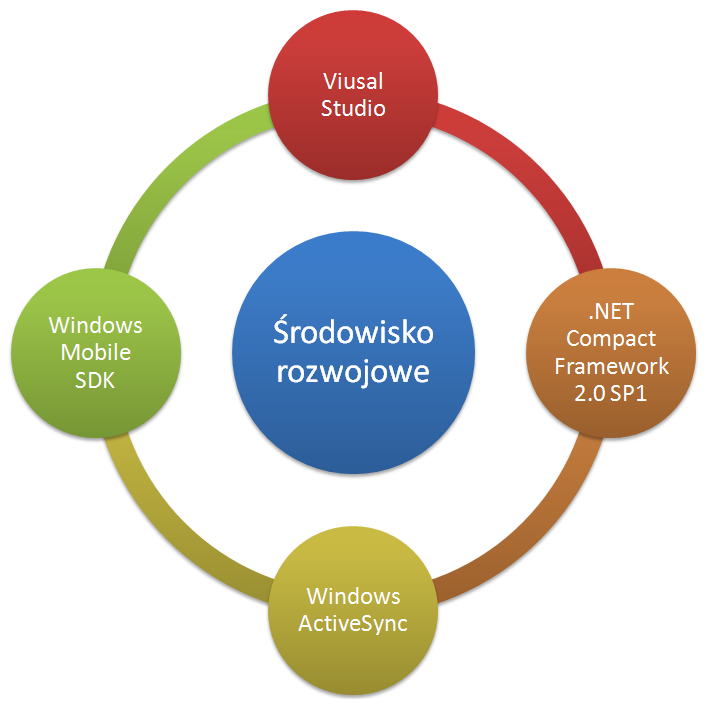
\includegraphics[height=100mm]{../images/ch03/wm_dev_env.png}
 \caption{Elementy składowe środowiska rozwojowego Windows Mobile}
 \label{fig:WMDevelopmentEnviroment}
\end{figure}

Przed rozpoczęciem przygody z tworzeniem aplikacji dla systemu Windows Mobile
konieczne jest zainstalowanie Microsoft Visual Studio. Zaleca się aby Visual
Studio było w wersji 2005 lub 2008. Niestety narzędzia umożliwiające rozwijanie
aplikacji mobilnych nie są poprawnie wykrywane przez Visual Studio 2010 oraz
poprzednie wydania w wersji Express. Dlatego też koniecznością jest instalacja
środowiska w wersji Standard lub Professional. Każda z tych wersji może zostać
pobrana w wersji czasowej ze stron firmy Microsoft lub w wersji pełnej z
MSDNAA\footnote{Microsoft Developer Network Academic Alliance - program firmy
Microsoft skierowany do studentów i pracowników naukowych w ramach którego
uczestnicy mogą pozyskać darmowe kopie oprogramowania firmy Microsoft}. Visual
Studio posłuży nam nie tylko do edycji kodu aplikacji ale pozwoli również w
prosty sposób budować, debugować oraz przygotować instalator finalnej wersji
aplikacji. Po poprawnym zainstalowaniu środowiska rozwojowego konieczne jest
pobranie i zainstalowanie dostępnych paczek serwisowych dostępnych dla wybranej
wersji Visual Studio. Pozwoli to uniknąć nieprzyjemnych niespodzianek podczas
instalacji bibliotek narzędziowych i późniejszej pracy.

Jeżeli posiadamy już zainstalowaną kopię Visual Studio możemy przystąpić do
instalacji narzędzi pomocniczych które pomogą nam w tworzeniu aplikacji. Pierwszą
niezbędną biblioteką jest .NET Compact Framework 2.0 SP1. Jest to zestaw narzędzi
wykorzystywanych do uruchamiania aplikacji na platformach opartych o Windows
Mobile. Aby ułatwić sobie proces budowania, debugowania i uruchamiania aplikacji
na urządzeniu konieczne jest zainstalowanie w systemie Windows ActiveSync. Dzięki
ActiveSync możliwe stanie się uruchamianie projektowanej aplikacji, bezpośrednio
z IDE, nie tylko na prawdziwym urządzeniu ale również emulatorze.

Ostatnim, ale i zarazem najważniejszym krokiem jest instalacja Windows Mobile
SDK\footnote{Software Development Kit - zestaw narzędzi programistycznych
niezbędnych do tworzenia aplikacji korzystających z funkcjonalności dostarczonej
przez daną bibliotekę}. Na stronach firmy Microsoft dostępne są dwie wersje SDK,
Standard oraz Professional. Wersja Standard zawiera w sobie tylko wsparcie dla
urządzeń z Windows Mobile Classic lub Standard natomiast wersja Professional
obejmuje wszystkie dostępne środowiska. Wybór SDK można sprowadzić do
następującej zasady. Jeżeli zamierzamy tworzyć oprogramowanie dla urządzeń
Smartphone bez ekranu dotykowego w zupełności wystarczy nam wersja standardowa.
Jeżeli natomiast planujemy napisane aplikacje uruchamiać na PocketPC lub
dotykowych SmartPhon'ach będziemy potrzebować bibliotek systemu Windows Mobile
Classic lub Professional, tak więc konieczne jest użycie SDK w wersji
Professional. Tak jak w przypadku Visual Studio, również tutaj zaleca się
instalację wszystkich dostępnych na stronie producenta aktualizacji i poprawek.
Jest to szczególnie istotne podczas pracy z emulatorami urządzeń. Po
zrealizowaniu tych kroków otrzymujemy w pełni funkcjonalne środowisko do rozwoju
aplikacji mobilnych dla urządzeń smartphone.

\subsubsection{Modele aplikacji}
Istnieje klika modeli rozwoju aplikacji dla Windows Mobile (rys. \ref{fig:WMDevelopmentModels}), a wybór docelowego
modelu został pozostawiony programiście. Pierwszy z nich służy do tworzenia
aplikacji w kodzie natywnym. Aplikacje pisane zgodnie z tym modelem cechują się
wysoką wydajnością, bezpośrednim dostępem do sprzętu oraz małym zużyciem zasobów.
Do rozwoju tego rodzaju aplikacji korzysta się z reguły ze środowiska do
rozwijania aplikacji z użyciem Embeded Visual C++. Główną wadą tego modelu jest
niska przenośność pomiędzy różnymi platformami zwłaszcza jeżeli aplikacja
korzysta z urządzeń specyficznych dla danego modelu urządzenia. Docelowo więc za
pomocą tego modelu tworzy się biblioteki i narzędzia ułatwiające tworzenie
bardziej skomplikowanych aplikacji. Jeżeli więc interesuje nas tworzenie
wysokopoziomowych aplikacji z GUI, skierowanych bezpośrednio do użytkowników,
zaleca się tworzenie tego typu aplikacji za pomocą kodu zarządzalnego z użyciem
takich języków jak C\# czy Visual Basic.

\begin{figure}[ht!]
 \centering 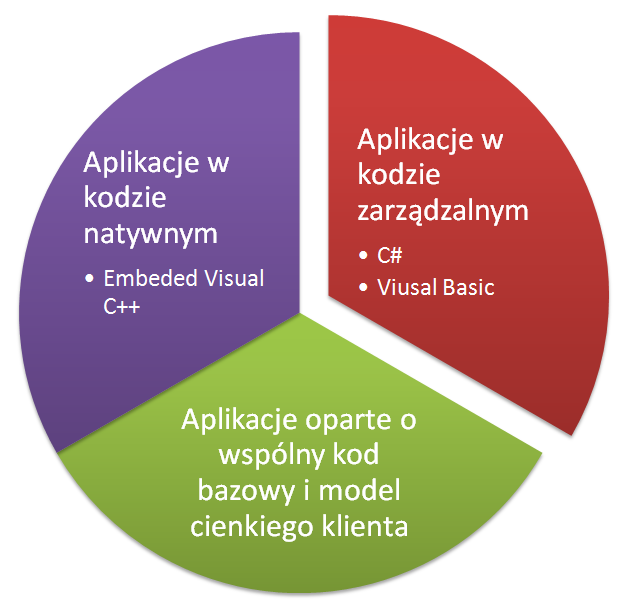
\includegraphics[height=85mm]{../images/ch03/wm_app_models.png}
 \caption{Modele tworzenia aplikacji dla Windows Mobile.}
 \label{fig:WMDevelopmentModels}
\end{figure}

Rozwijanie aplikacji w oparciu o kod zarządzalny pozwala na stworzenie programu
który będzie mógł w pełni wykorzystywać możliwości oferowane przez Microsoft .NET
Compact Framework. Umożliwia to programiście tworzenie rozproszonych systemów
mobilnych pracujących zarówno w modelu ze stałym połączeniem jak i bez. Spora
część narzędzi dostępnych w ramach .NET Compact Framework jest również
wykorzystywana do rozwoju aplikacji na komputery stacjonarne. Biblioteka została
zaprojektowana docelowo na urządzenia o ograniczonych zasobach co w połączeniu z
możliwościami języków z rodziny .NET oraz integracją z Visual Studio daje nam
profesjonalny zestaw narzędzi do tworzenia aplikacji mobilnych.

Trzecim modelem tworzenia programów pod Windows Mobile jest wykorzystywanie kodu
serwera do pracy z wieloma różnymi typami urządzeń poprzez jeden wspólny kod
bazowy i model cienkiego klienta. Oczywiście tego typu podejście ma sens jedynie
gdy możemy zagwarantować stabilny kanał komunikacyjny pomiędzy urządzeniem
klienta, a serwerem. Każdy z przedstawionych modeli idealnie sprawdza się jeżeli
tylko w prawidłowy sposób wybierzemy model najbardziej odpowiadający potrzebom
naszej aplikacji.
\subsubsection{Graficzny interfejs użytkownika}
Dzięki wygodnemu systemowi projektowania GUI dostępnego w Visual Studio, tworzenie
interfejsu użytkownika dla platformy mobilnej jest niemal tak proste jak w
przypadku tradycyjnych aplikacji, a jedyną różnicą jest ilość i rodzaj dostępnych
kontrolek. Różnice te wynikają z faktu iż niektóre urządzenia mobilne posiadają
ekrany dotykowe, a inne nie. Co za tym idzie, rozwój interfejsu użytkownika staje
się bardziej skomplikowany zwłaszcza jeżeli interesuje nas rozwój aplikacji
wspólnej dla obydwu platform sprzętowych. W tym miejscu nie może zabraknąć
informacji, że oprogramowanie zbudowane dla PocketPC nie uruchomi się na
urządzeniach SmartPhone natomiast sytuacja odwrotna jest możliwa do momentu w
którym aplikacja nie zacznie korzystać ze specyficznych funkcji SmartPhone.
Naturalnym stanem rzeczy wydaje się fakt, iż wiele funkcji i komponentów
graficznych znanych z aplikacji desktopowych zostało usunięte z bibliotek Windows
Mobile, aby zapewnić jej wydajność i niewielki rozmiar. Dlatego też pozostawiono
tylko niezbędne, najprostsze komponenty. Ponieważ wydajność  i zasoby pamięciowe
urządzeń stale rosną, również ilość narzędzi dostępnych w SDK jest systematycznie
zwiększana, a co za tym idzie różnice pomiędzy kolejnymi wersjami .NET Compact
Framework są bardzo duże. Dlatego też posiadanie jak najbardziej aktualnej wersji
SDK ma niebagatelne znaczenie dla wygody tworzenia aplikacji. Podsumowując, rozwój
GUI dla platformy mobilnej nie różni się bardzo od tworzenia interfejsu
użytkownika dla aplikacji dekstopowej. Istnieje również możliwość rozwijania GUI
w oparciu o silniki 3D. W chwili obecnych dostępne są takie rozwiązania jak GAPI
(Game API), OpenGL ES (Embeded Systems), Open VG (Vector Grapics). Jednakże
rozwój takich aplikacji jest niezwykle trudny gdyż wymaga od programisty
tworzenia maksymalnie optymalnego kodu, ze względu na ograniczone możliwości
niektórych urządzeń.

\subsubsection{Komunikacja}
Nowoczesne urządzenia mobilne posiadają szeroką gamę możliwości komunikacyjnych (rys. \ref{fig:WMCommunicationAPI}).
Posiadają one dostęp do szybkich sieci bezprzewodowych w standardzie 802.11 WiFi.
Umożliwiają one również komunikację za pomocą portu podczerwieni, bluetooth czy
USB. Podejmując decyzję na temat wyboru kanału komunikacji należy brać pod uwagę
nie tylko parametry techniczne, ale również liczbę standardów i protokołów
dostępnych dla danego kanału komunikacji. Firma Microsoft dostarcza szereg
interfejsów programistycznych (API) umożliwiających niemal błyskawiczny dostęp do
funkcji komunikacyjnych urządzenia. AcitveSync API dostarcza funkcjonalność
umożliwiającą komunikację za pomocą protokołu synchronizacji. Natomiast Bluetooth
API dostarcza zestaw narzędzi umożliwiających nawiązywanie komunikacji
bezprzewodowej pomiędzy telefonami jak i urządzeniami peryferyjnymi.

\begin{figure}[h!]
 \centering 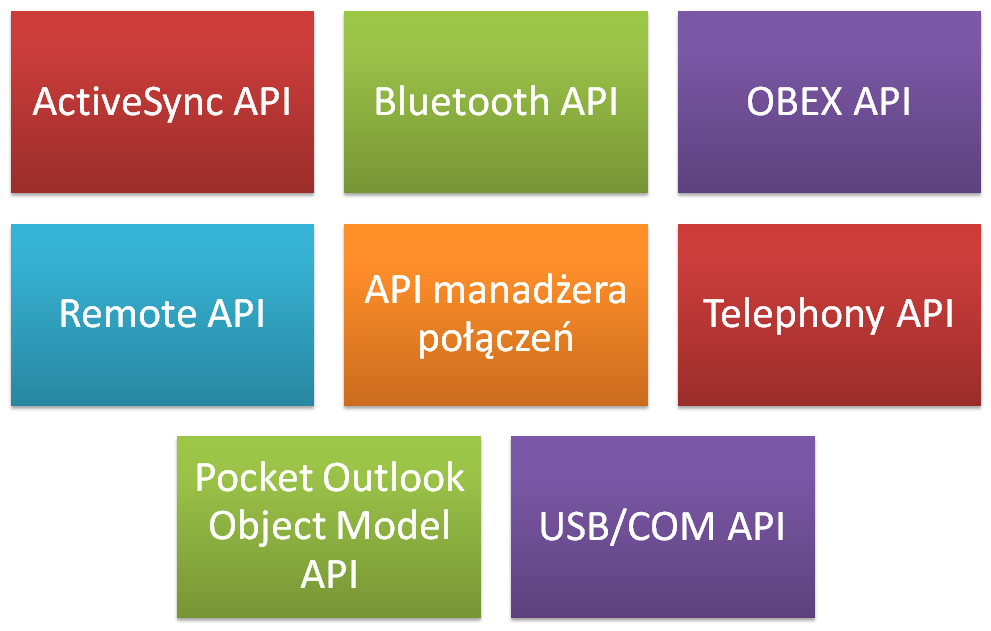
\includegraphics[height=85mm]{../images/ch03/wm_comm_api.png}
 \caption{Lista dostępnych na platformie Windows Mobile API komunikacyjnych}
 \label{fig:WMCommunicationAPI}
\end{figure}

API Managera połączeń dostarcza zestaw usług umożliwiających automatyzację
procesu nawiązywania połączenia oraz zarządzanie ich aktywnością. API wymiany
obiektów (OBEX API) dostarcza funkcjonalność umożliwiającą wymianę danych
pomiędzy urządzeniami za pomocą efektywnego, kompaktowego protokołu binarnego
dedykowanego dla urządzeń z ograniczonymi zasobami. Remote API (RAPI) dostarcza
funkcję do zarządzania oraz zdalnego wywoływania metod po stronie urządzenia
klienta. Dostępne są m.in. funkcje dostępu do rejestru, plików, bazy danych czy
też konfiguracji urządzenia. Najważniejszą funkcjonalnością jest jednak możliwość
zdalnego wywoływania procedur. Za pomocą funkcji CeRapiInvoke() przesyłamy do
urządzenia nazwę biblioteki dynamicznej wraz z nazwą metody która ma zostać
wywołana na urządzeniu mobilnym. Kolejnym zestawem narzędzi jest Pocket Outlook
Object Model API. Dostarcza ono funkcje do zarządzania obiektami Pocket Outlook, co
umożliwia synchronizację zadań, kalendarza czy kontaktów za pomocą prostego i
intuicyjnego interfejsu. Dostępne jest również Telephony API (TAPI) które zawiera
w sobie biblioteki umożliwiające zarządzanie kartą SIM oraz wiadomościami SMS.
TAPI udostępnia również zestaw funkcji umożliwiających dostęp do funkcji
telefonowania oraz protokołu WAP. Nie zabrakło również narzędzi do pracy z
portami USB oraz COM. Część z dostępnych portów COM jest zarezerwowana dla
urządzeń wewnętrznych, ale pozostałe dostępne są do pełnej dyspozycji
użytkownika.

\subsubsection{Debugowanie}
Microsoft Visual Studio umożliwia debugowanie aplikacji działających pod kontrolą
Windows Mobile niemal w taki sam sposób jak ma to miejsce w przypadku
tradycyjnych aplikacji desktopowych. Ponadto programista ma do swojej dyspozycji
następujące narzędzia: emulator, panel zarządzania emulowanymi urządzeniami,
panel punktów przerwań i wątków. Niestety w Visual Studio nie uda się nam
jednocześnie debugować kodu natywnego i zarządzalnego. Możliwe jest natomiast
uruchomienie zarówno projektu napisanego w Visual C++ jak i projektu opartego o
kod zarządzalny, a dzięki funkcjonalności ,,Dołącz do procesu'' możliwe jest
zdalne dołączenie się i monitorowanie procesu działającego na urządzeniu lub
emulatorze urządzenia. Narzędziem umożliwiającym komunikację pomiędzy urządzeniem
a systemem jest ActiveSync instalowany wraz ze środowiskiem rozwojowym. Za pomocą
narzędzia ActiveSync możemy łączyć się nie tylko z rzeczywistymi urządzeniami ale
również z emulatorami. Umożliwia to pełną wirtualizację urządzeń mobilnych i
znacznie ułatwia testowanie funkcjonalności zwłaszcza pomiędzy różnymi
platformami urządzeń (SmartPhone, PocketPC). Jedynym ograniczeniem tego procesu
jest możliwość utrzymania tylko jednego aktywnego połączenia co uniemożliwia
debugowanie na wielu urządzeniach jednocześnie. Co więcej, Visual Studio umożliwia
debugowanie jedynie aplikacji stworzonej przez programistę, nie możliwe jest z
poziomu IDE debugowanie aplikacji i usług systemowych działających na urządzeniu.
Do tego typu debugowania konieczne byłoby zbudowanie własnej wersji systemu
Windows Mobile przy użyciu Platform Buildera. Narzędzie to umożliwia również
tworzenie własnego SDK dla Visual Studio i platformy Windows CE. Dodatkową
możliwością dostępną z poziomu emulatora jest emulowanie połączenia z siecią GSM
oraz wsparcie dla GPS. Umożliwia to testowanie, debugowanie i rozwijanie
szerokiego spektrum aplikacji bez konieczności posiadania urządzenia fizycznie.

\subsection{Środowisko uruchomieniowe aplikacji mobilnej}
Docelowym środowiskiem na którym uruchamiana będzie aplikacja sterująca robotem
Dark Explorer będą urządzenia działające pod kontrolą systemu Windows Mobile.
Jedynym wymaganiem stawianym przed urządzeniem na którym podjęta zostanie próba
uruchomienia aplikacji jest posiadanie uprzednio zainstalowanej biblioteki .NET
Compact Framework w wersji co najmniej 2.0 SP1. Wersję instalacyjną biblioteki
dla której były przeprowadzane testy można znaleźć na dołączonej do pracy
płycie. 

\subsubsection{Instalacja aplikacji sterującej}
Przed przystąpieniem do korzystania z mobilnej aplikacji sterującej konieczne
jest jej zainstalowanie na urządzeniu za pomocą którego użytkownik chciałby
komunikować się z robotem mobilnym. Aby tego dokonać konieczne jest skopiowanie
pliku instalatora do pamięci telefonu. Po zakończeniu procesu kopiowania za
pomocą menadżera plików zainstalowanego w telefonie uruchamiamy instalator
aplikacji zgodnie z rysunkiem \ref{fig:wm-install-1}. W przypadku gdy dokonujemy aktualizacji wersji
aplikacji instalator poinformuje użytkownika o wykrytej wersji aplikacji i będzie
wymagał potwierdzenia przed usunięciem poprzedniej wersji i kontynuacją
instalacji obecnej wersji. Komunikat którego może się spodziewać użytkownik
widoczny jest na zdjęciu \ref{fig:wm-install-3}. Kolejnym etapem instalacji
będzie wybór katalogu docelowego w którym zainstalowana zostanie aplikacja
(rys. \ref{fig:wm-install-4}). Po~rozpoczęciu pracy instalator będzie informował
użytkownika o stanie procesu za pomocą widocznego na rysunku
\ref{fig:wm-install-5} paska postępu. Instalacja może zająć od kilku do kilku
dziesięciu sekund w zależności od aktulanego obciążenia i konfiguracji
sprzętowej telefonu. Poprawne zakończenie instalacji zostanie potwierdzone poprzez wyświetlenie
komunikatu widocznego na rysunku \ref{fig:wm-install-6}. Po poprawnym
zainstalowaniu aplikacji konieczne jest jeszcze skonfigurowanie połączenia
bluetooth, aby program sterujący potrafił z niego poprawnie skorzystać. 
W~tym celu należy uruchomić moduł bluetooth zarówno w telefonie jak i robocie.
Następnie należy sparować urządzenia, aby umożliwić im bezpośrednią wymianę
danych bez konieczności potwierdzania przesłania każdego komunikatu. Domyślnym
kodem potrzebnym do nawiązania połącznia bluetooth jest kod ,,0000''. Kolejnym
etapem konfiguracji jest uruchomienie usługi komunikacji za pomocą
protokołu RFCOMM oraz stworzenie nowego portu wychodzącego poprzez który
przesyłane będą dane pomiędzy robotem, a~urządzeniem sterującym. Wszystkie
wspomniane kroki konfiguracyjne zaprezentowane są kolejno na rysunkach
\ref{fig:wm-config-1}, \ref{fig:wm-config-2} oraz \ref{fig:wm-config-3}. Po
zakończeniu tego etapu możliwe jest już rozpoczęcie korzystania z wszystkich
możliwości oferowanych przez aplikację.

 \begin{figure}[h!]
 \centering
 \subfloat[Uruchomienie instalatora]{\label{fig:wm-install-1}
 	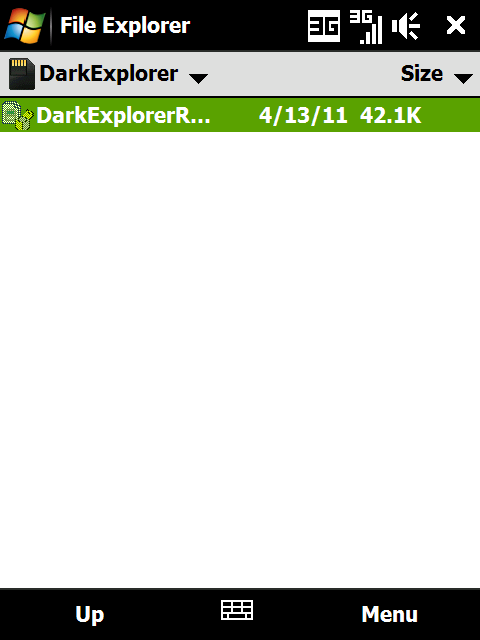
\includegraphics[width=0.30\textwidth]{../images/ch03/wm-install-1.png}}
 \subfloat[Przygotowanie instalacji]{\label{fig:wm-install-2}
 	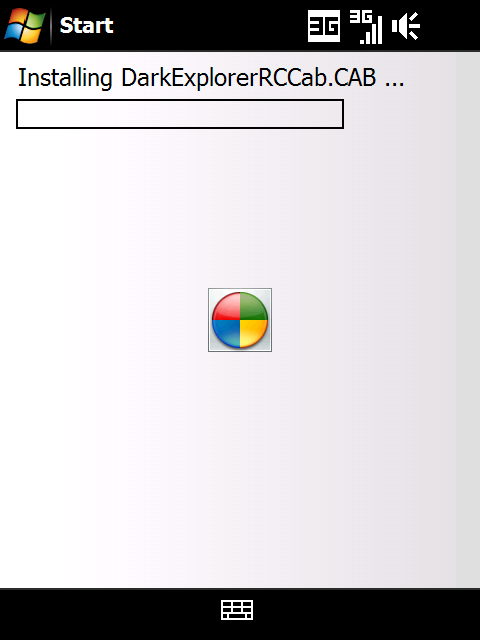
\includegraphics[width=0.30\textwidth]{../images/ch03/wm-install-3.png}}
 \subfloat[Potwierdzanie reinstalacji]{\label{fig:wm-install-3}
 	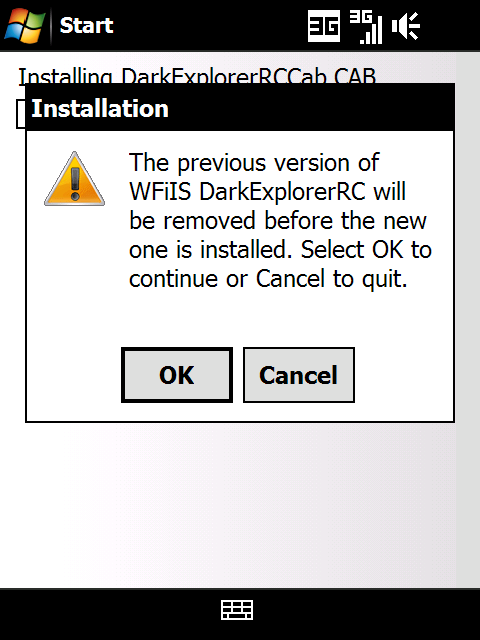
\includegraphics[width=0.30\textwidth]{../images/ch03/wm-install-2.png}} 
 	\hfill \\
 \subfloat[Wybór miejsca instalacji]{\label{fig:wm-install-4}
 	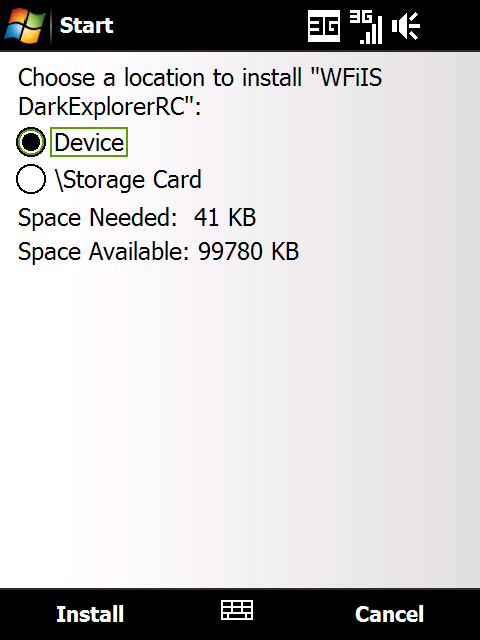
\includegraphics[width=0.30\textwidth]{../images/ch03/wm-install-4.png}}
 \subfloat[Instalator w trakcie działania]{\label{fig:wm-install-5}
 	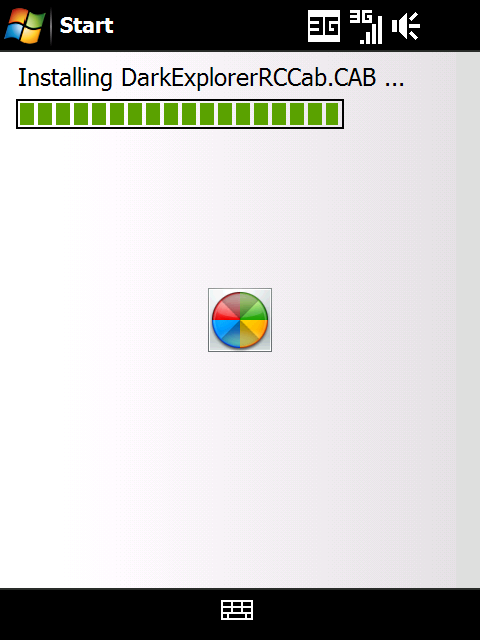
\includegraphics[width=0.30\textwidth]{../images/ch03/wm-install-5.png}}
 \subfloat[Poprawne ukończenie instalacji]{\label{fig:wm-install-6}
 	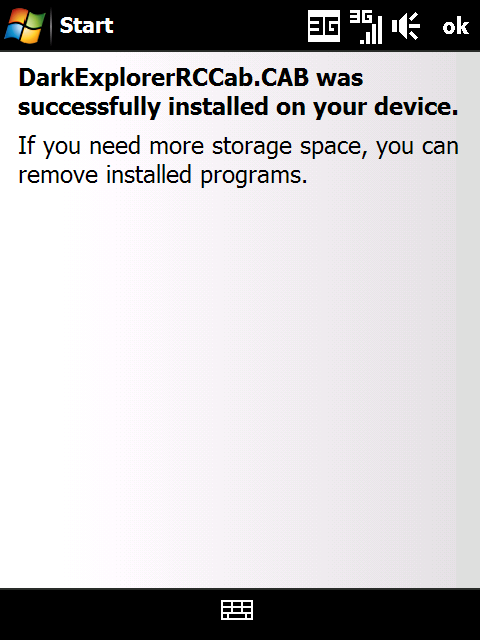
\includegraphics[width=0.30\textwidth]{../images/ch03/wm-install-6.png}}
 		\hfill \\
 \subfloat[Parowanie urządzenia]{\label{fig:wm-config-1}
 	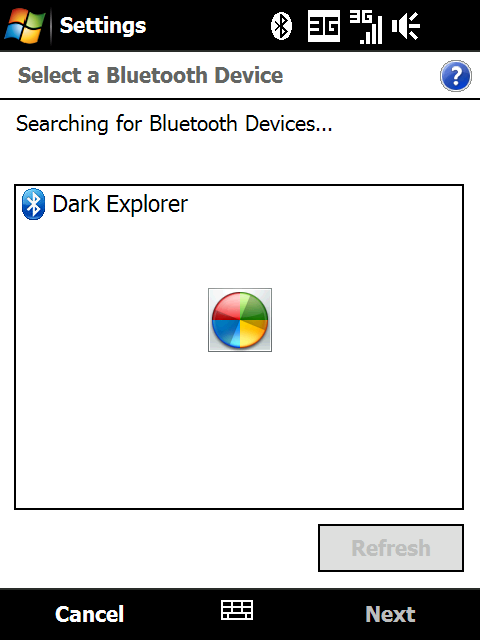
\includegraphics[width=0.30\textwidth]{../images/ch03/wm-config-2.png}}
 \subfloat[Uruchamianie usługi]{\label{fig:wm-config-2}
 	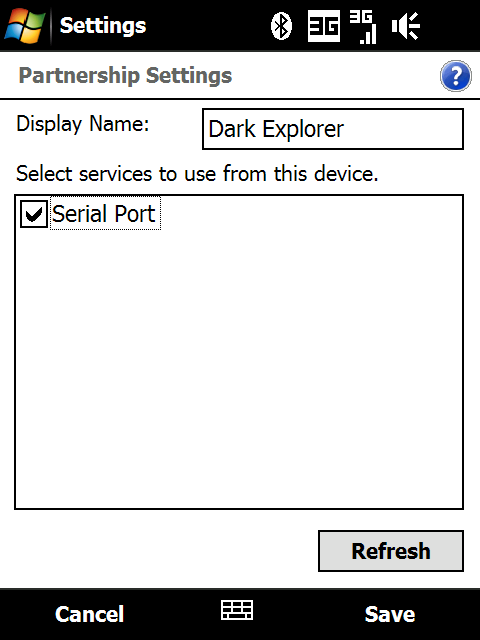
\includegraphics[width=0.30\textwidth]{../images/ch03/wm-config-4.png}}
 \subfloat[Konfiguracja portu COM]{\label{fig:wm-config-3}
 	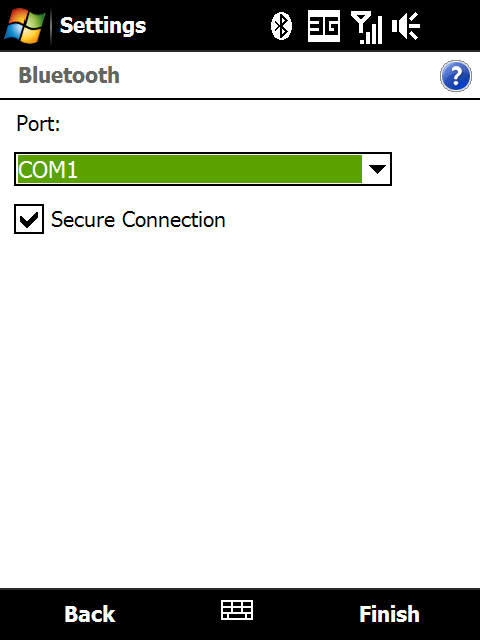
\includegraphics[width=0.30\textwidth]{../images/ch03/wm-config-0.png}}
 \caption{Kroki wymagane do przeprowadzenia poprawnej instalacji i konfiguracji mobilnej aplikacji sterującej}
 \label{fig:wm-install&conf}
\end{figure}

\subsubsection{Uruchomienie aplikacji sterującej}
Jeżeli posiadamy już zainstalowaną i skonfigurowaną aplikację sterującą to
możemy rozpocząć korzystanie z jej możliwości. W tym celu należy włączyć robota
i uruchomić moduł bluetooth dostępny w telefonie. Następnie na liście dostępnych
aplikacji należy odszukać program pod nazwą ,,Dark Explorer RC'' ikona programu
widoczna jest na rysunku \ref{fig:wm-app-2}. Wybierając program z listy
zainicjujemy proces jego uruchamiania. Po załadowaniu wszystkich komponentów
aplikacji na ekranie wyświetli się okno główne aplikacji widoczne na rysunku
\ref{fig:wm-app-3}. Aby uprościć dostęp do funkcji programu zostały one
wszystkie zebrane w menu dostępnym w lewym dolnym rogu aplikacji. Wszystkie
dostępne opcje pogrupowano pod względem tematycznym, tak aby nawet użytkownik
uruchamiający aplikację po raz pierwszy nie miał trudności z odszukaniem
interesujących go funkcji. 

 \begin{figure}[h!]
 \centering
 \subfloat[Uruchomienie bluetooth]{\label{fig:wm-app-1}
 	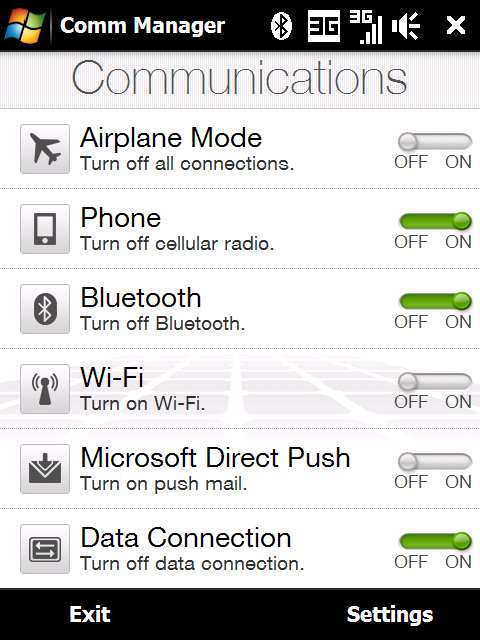
\includegraphics[width=0.30\textwidth]{../images/ch03/wm-app-0.png}}
 \subfloat[Ikona startowa]{\label{fig:wm-app-2}
 	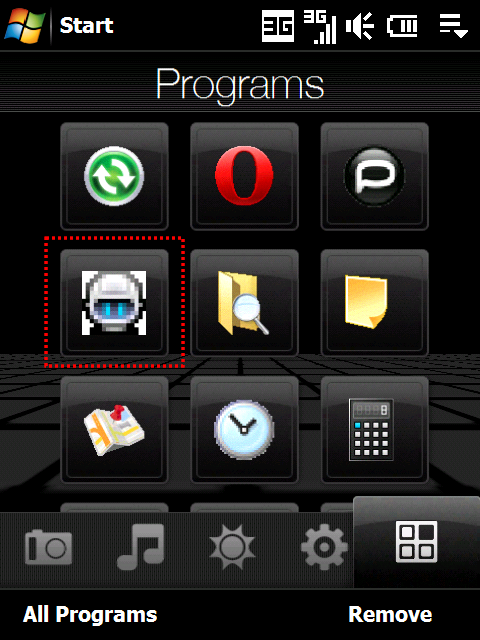
\includegraphics[width=0.30\textwidth]{../images/ch03/wm-app-1.png}}
 \subfloat[Okno główne programu]{\label{fig:wm-app-3}
 	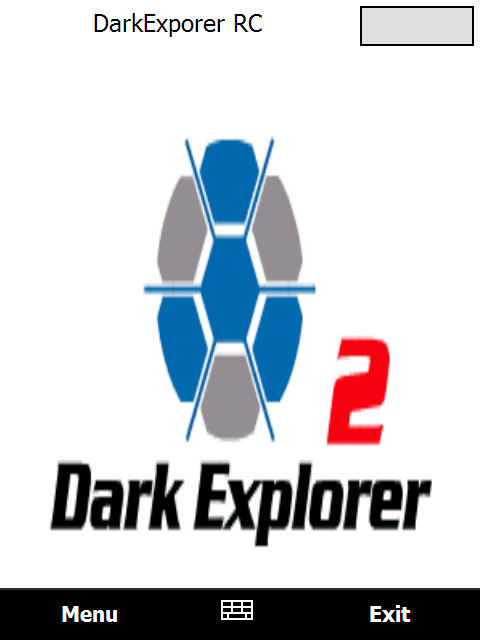
\includegraphics[width=0.30\textwidth]{../images/ch03/wm-app-2.png}} 
 \caption{Uruchomienie mobilnej aplikacji sterującej}
 \label{fig:wm-run}
\end{figure}

Aby uczynić aplikację jeszcze bardziej przyjazną użytkownikowi część funkcji
dostępna jest również pod sprzętowymi przyciskami telefonu. Dobrym przykładem
tego rodzaju funkcji jest sterowanie kierunkiem jazdy robota. Dostęp do tej
funkcjonalności można uzyskać bezpośrednio za pomocą przycisków strzałek
góra, dół, prawo, lewo. Ponad to naciskając przycisk środkowy użytkownik ma
możliwość pobrania danych z kamery zgodnie z aktualną konfiguracją aplikacji.
Dodatkowym atutem programu jest możliwość sterownia kierunkiem jazdy robota za
pomocą akcelerometru jeżeli urządzenie mobilne jest w takowy wyposażone.
Aktualny stan robota oraz aplikacji prezentowany jest w pasku statusu widocznym
u góry okna głównego aplikacji. Pozwala to użytkownikowi na bieżąco monitorować
nie tylko stan aplikacji ale również to co w chwili obecnej dzieje się na
robocie.